% set 0.5 inch indentation
% \setlength{\parindent}{0.5in}
\setlength{\parindent}{0pt} 
% set paragraph space = 0 space
\setlength{\parskip}{0mm}
% set line space 1.5
\setlength{\baselineskip}{1.6em}

\chapter{EXPERIMENTAL RESULTS}
\label{ch:results}
In this chapter, two experiments comprising simulations with three drones and a real world experiment with one drone are described. 

\section{Real World Experiment}
To test the automated system, an experiment was run in the Energy Park behind CSIM building. The site was chosen as it has structures which will help SURF descriptors recognize features. 

\begin{figure} 
	\centering
	\caption[Drone used in experiment.]{\small 
		The drone used in real world experiment. (a) Top view. (b) Side View. The weight of the drone is 1.8 kilogram. }
	\subfloat[]{%
		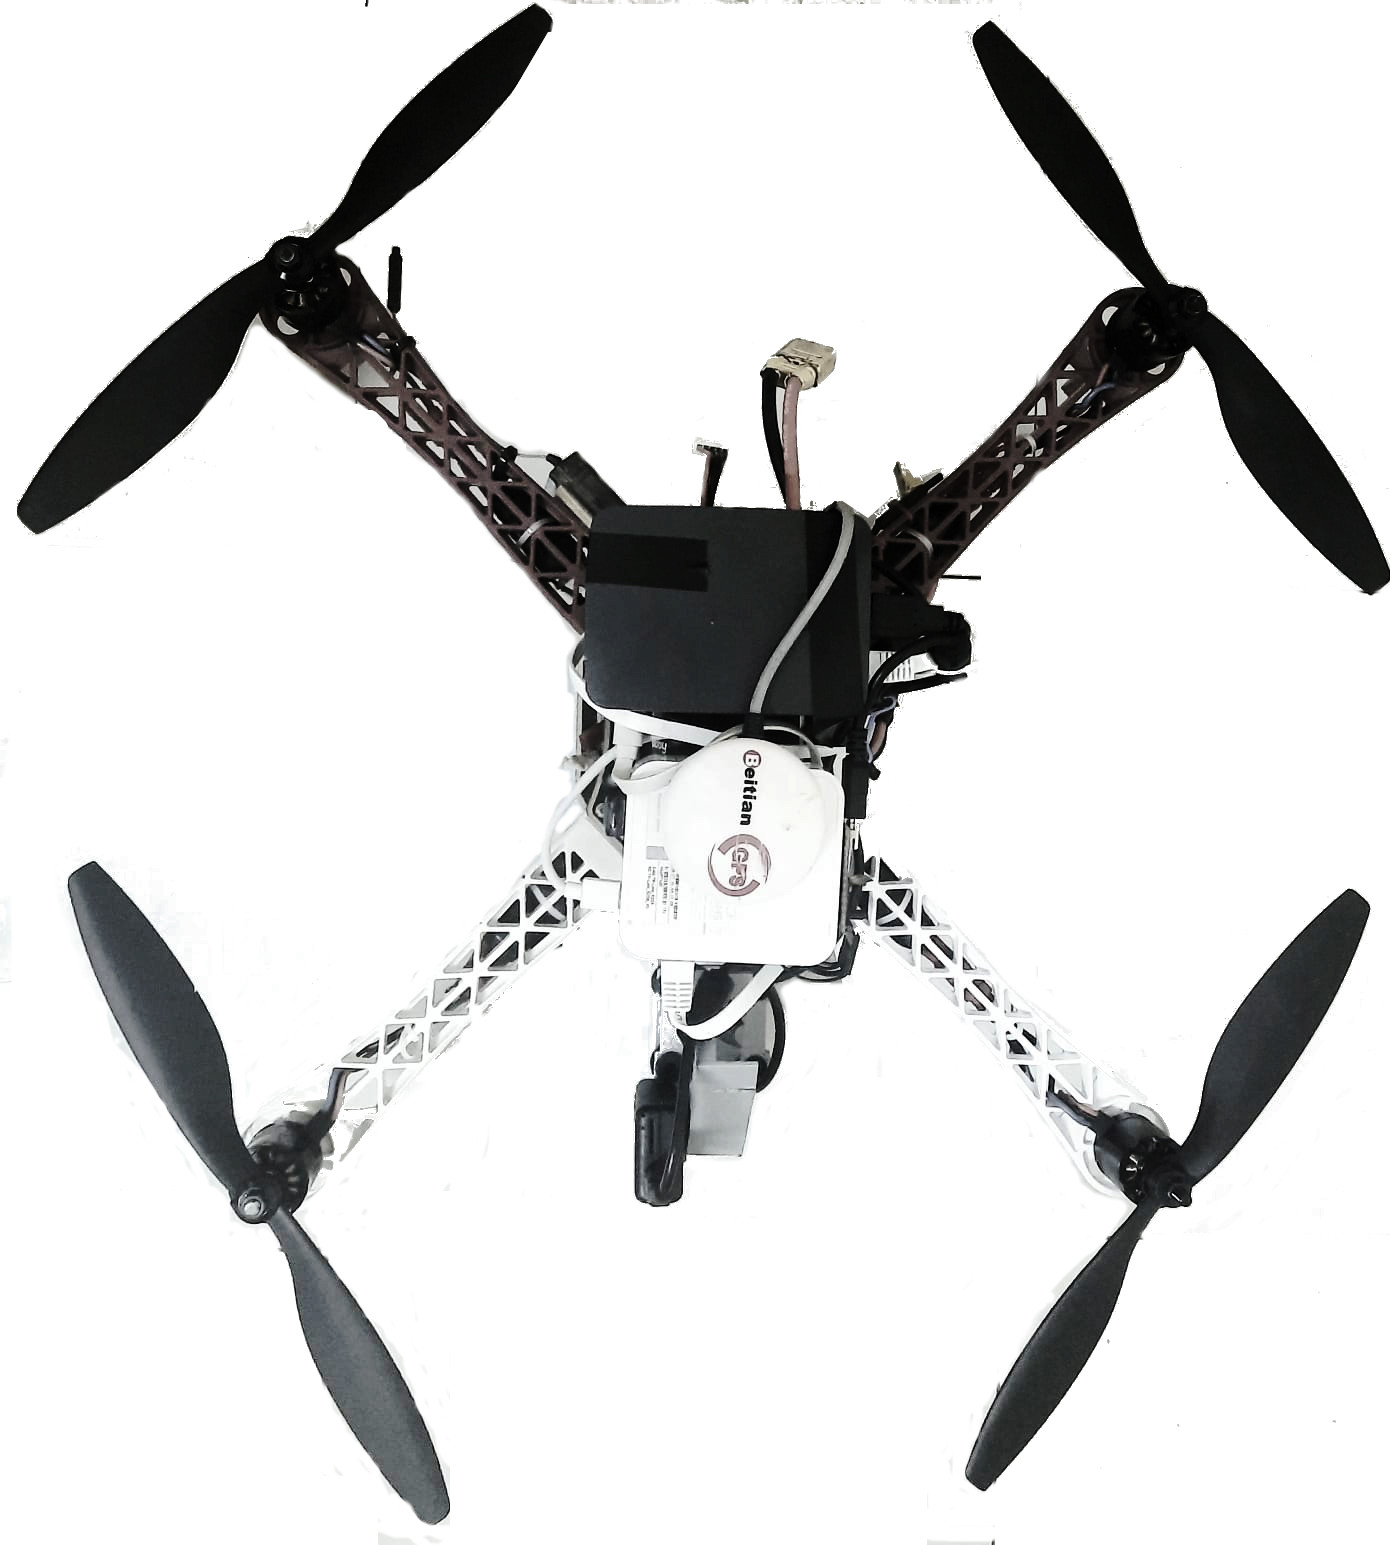
\includegraphics[width=3in]{figures/methodology/drone-top}
	}	
	\subfloat[]{%
		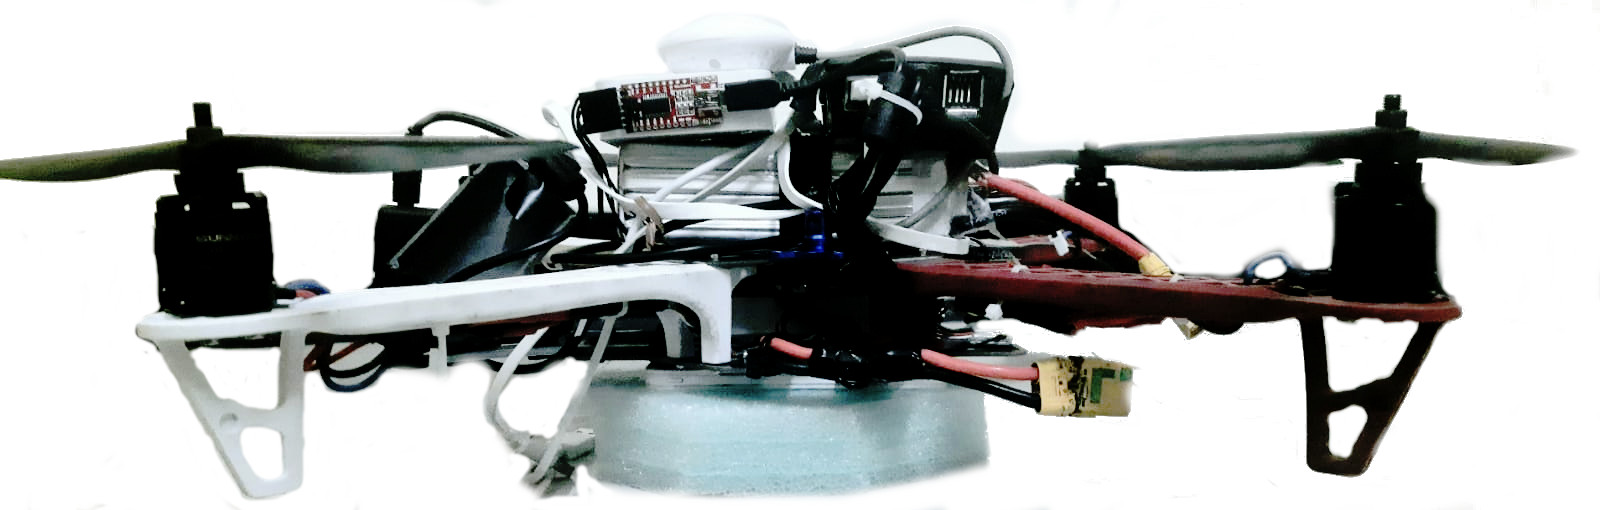
\includegraphics[width=3in]{figures/methodology/drone-side}
	}
	\label{fig:real-drone}
\end{figure}


\subsection{Mesh Network}

The mesh network consists of two wireless mesh routers running OpenWrt. Both of the routers are dual channel 2.5/5 GHz's routers with two radios. The GCS wireless router is a Netgear router (Figure~\ref{fig:gcs-router}). The GCS laptop is connected to the router via 2.5GHz WiFi network with SSID UAV01\_01. The TP-Link mobile wireless router (Figure~\ref{fig:mobile-router}) mounted on the drone is connected to the companion Raspberry Pi via Ethernet. The SSID of the mesh network is UAV01\_MESH5G and is running on 5 GHz channel. Figure~\ref{fig:mesh-network-real-world} shows the network infrastructure used.

The GCS laptop and companion are not mesh clients but are connected to different networks. Route between the GCS laptop and companion Raspberry Pi is achieved by using OSLR Host and network association (HNA) message to allow connection to these networks. Since GCS laptop is connected to different subnet than the Raspberry Pi, a route \texttt{\$ sudo route add -net 192.168.41.0/24 gw 192.168.40.1 wlp0s20f3} has to be added manually in the GCS laptop to divert the packet for the Raspberry Pi's subnet via the wireless LAN interface of the GCS to the the mesh network.

The IP assignment for different nodes in the network is given in Table~\ref{tab:network-assignment}. The OSLR messages' interval and validity for the GCS wireless mesh router and the mobile wireless mesh router is given in Table~\ref{tab:gcs-olsr-setting}.


\begin{table}[t]
	\caption[IP assignment for real world experiment.]{\small IP assignment for real world experiment. Laptop and Raspberry Pi have local network addresses assigned by the respective routers they are connected to, but all communication is through the mesh network with the routers as gateways.}
	\begin{center}
		\begin{tabular}{c|c|c|c}
			\hline Node & IP Address & Subnet & OSLR Interface IP\\ \hline \hline
			GCS Wireless Router & 192.168.40.1 &  192.168.40.1/24 & 192.168.30.1 \\ \hline
			Mobile Wireless Router & 192.168.41.1 & 192.168.41.1/24 & 192.168.30.2   \\ \hline 
			GCS Laptop & 192.168.40.216 & 192.168.40.1/24 & -  \\ \hline 
			Companion Raspberry Pi & 192.168.41.200 & 192.168.41.1/24 & - \\ \hline
		\end{tabular}
	\end{center}
	\label{tab:network-assignment}
\end{table} 


\begin{figure}
	\centering
	\caption[Network infrastructure for real world experiment.]{\small Network infrastructure for real world experiment.} 
	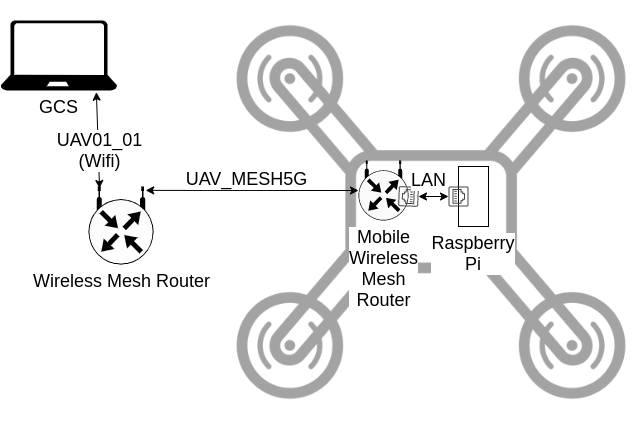
\includegraphics[width=5in]{figures/experiment/real-world-network}
	\label{fig:mesh-network-real-world}
\end{figure}

\begin{figure}
	\centering
	\caption[Wireless routers used in experiment.]{\small 
		Routers used for the experiment. (a) Netgear wireless router for the GCS. (b) TP-Link mobile wireless router mounted on the drone. }
	\subfloat[]{%
		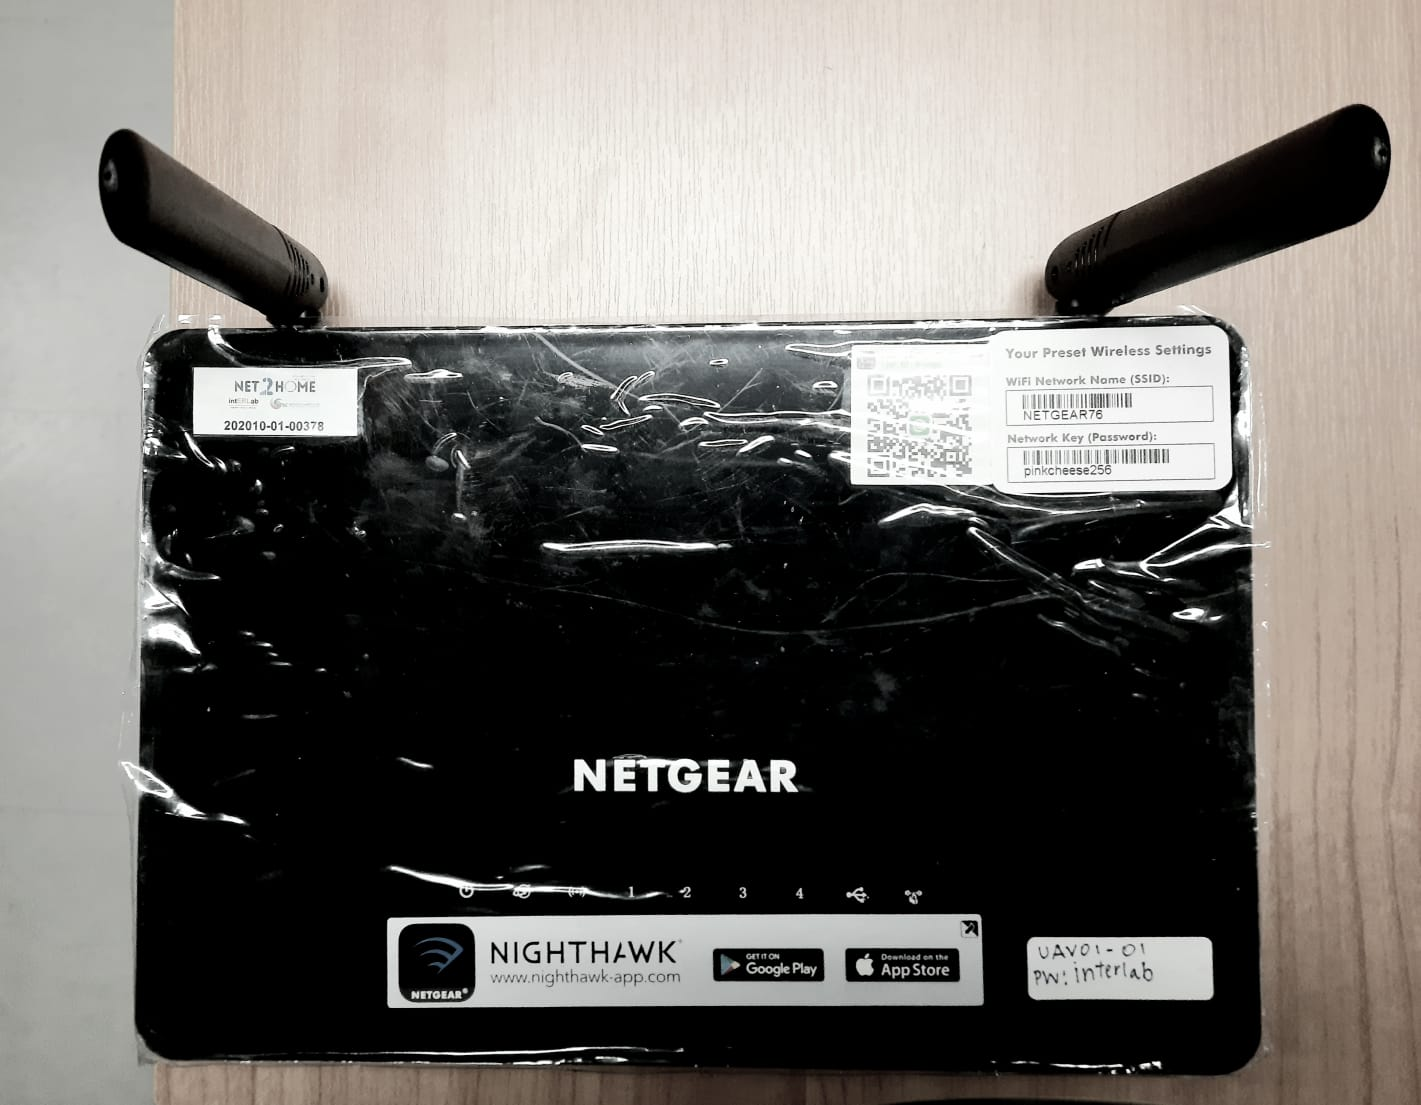
\includegraphics[width=3in]{figures/experiment/router2-mesh}
		\label{fig:gcs-router}
	}
	\subfloat[]{%
		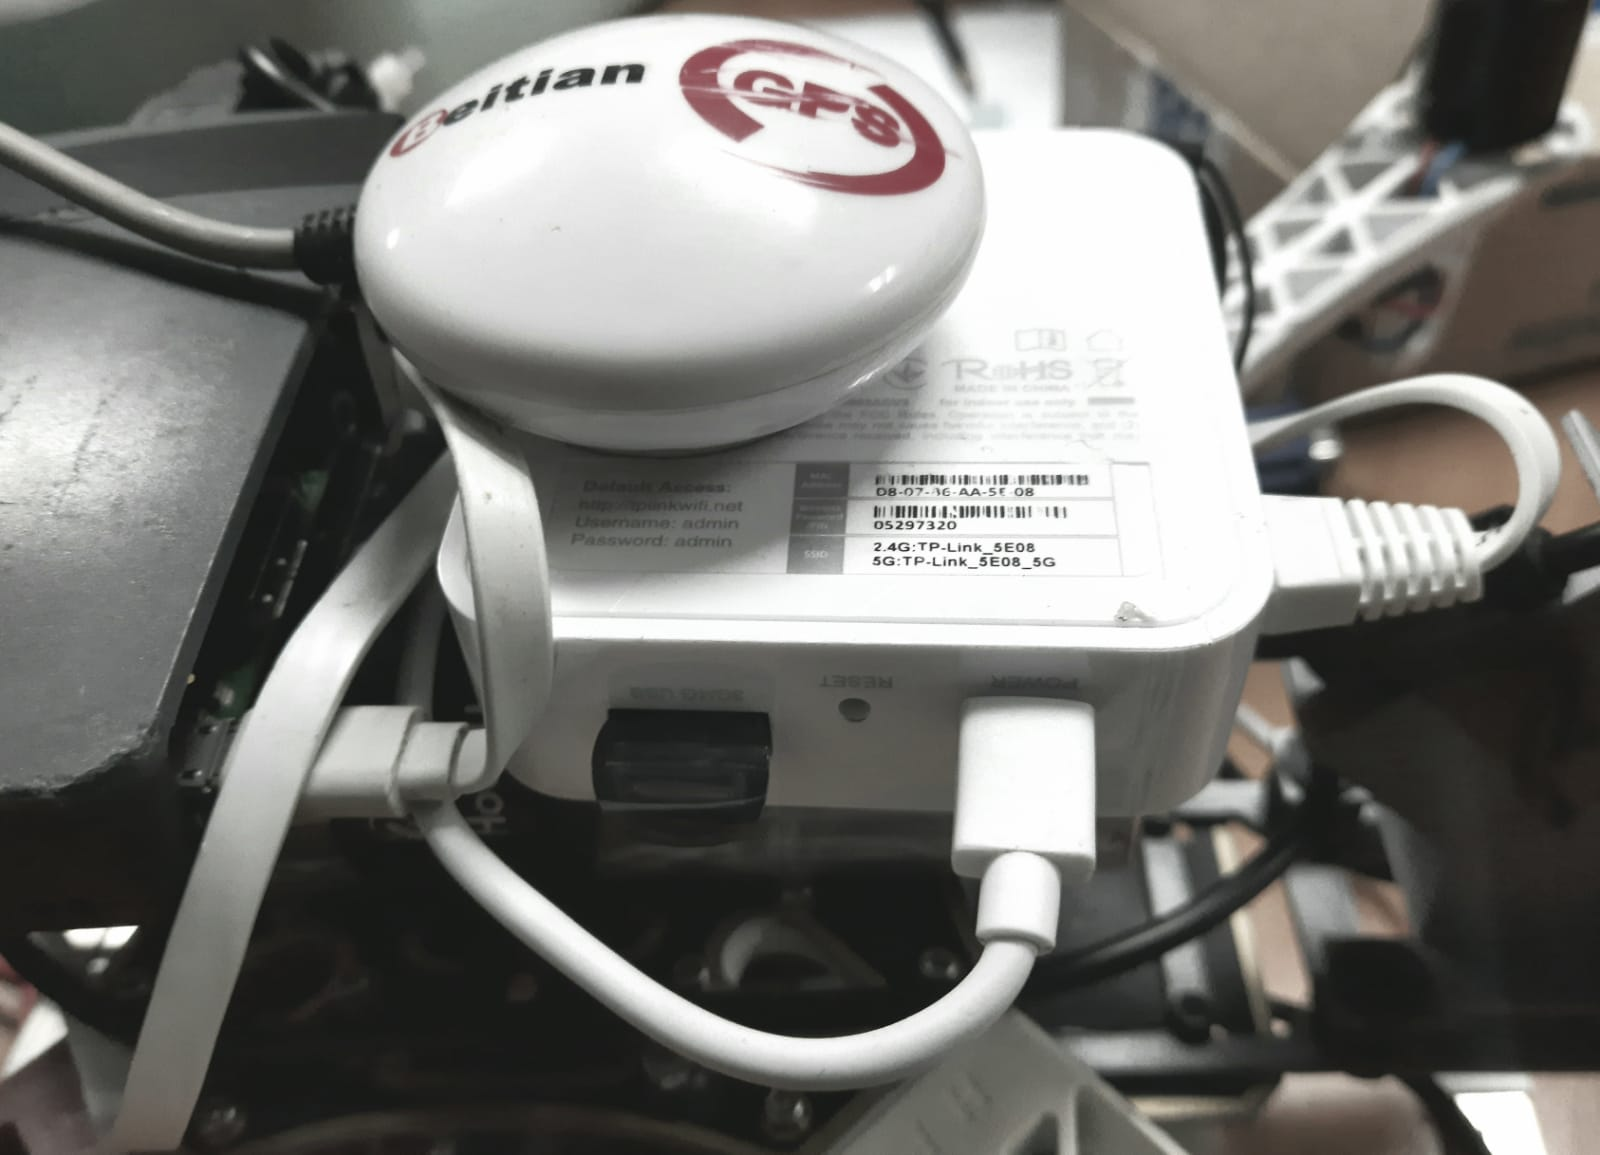
\includegraphics[width=3in]{figures/experiment/router1-mesh}%
		\label{fig:mobile-router}
	}
	
	\label{fig:real-routers}
\end{figure}


\begin{table}[h!]
	\caption[OLSR messsages' interval and validity parameters for real world experiment.]{OLSR messages' interval and validity parameters for real world experiment.}
	\begin{center}
		\begin{tabular}{c|c|c}
			\hline Message & Interval & Validity Time \\ \hline \hline
			Hello & 5 sec &  40 sec \\ \hline
			TC & 2 sec & 256 sec \\ \hline 
			MID & 18 sec & 324 sec  \\ \hline 
			HNA & 18 sec & 108 sec \\ \hline
		\end{tabular}
	\end{center}
	\label{tab:gcs-olsr-setting}
\end{table}


\subsection{Automated Planning}

For planning the path, the operational altitude was set at 20 meters, the grid size was set at 10 meters and the mesh range was set to 40 meters. The approximate area of coverage was 35 by 40 meters. The results of planning is given in Table~\ref{tab:real-world-planning}. The viewpoints and the path generated is shown is Figure~\ref{fig:real-path}. The optimum length of the path for the viewpoints is sixteen, but the planner provided a path of eighteen viewpoints which resulted in the drone visiting two viewpoints more than once. The length of the path was 178.2 meters.
\begin{table}[t]
	\caption[Result of \texttt{pegasus\_planner} in real world experiment.]{\small Result of \texttt{pegasus\_planner} in real world experiment.}
	\begin{center}
		\begin{tabular}{c|c|c|c}
			\hline Type & Number of Drones & Viewpoints Generated & Path Size \\ \hline \hline
			Real Experiment & 1 & 16 & 18 \\ \hline
		\end{tabular}
	\end{center}
	\label{tab:real-world-planning}
\end{table} 


\begin{figure}
	\centering
	\caption[Path generated for real world experiment.]{\small Path generated for real world experiment.} 
	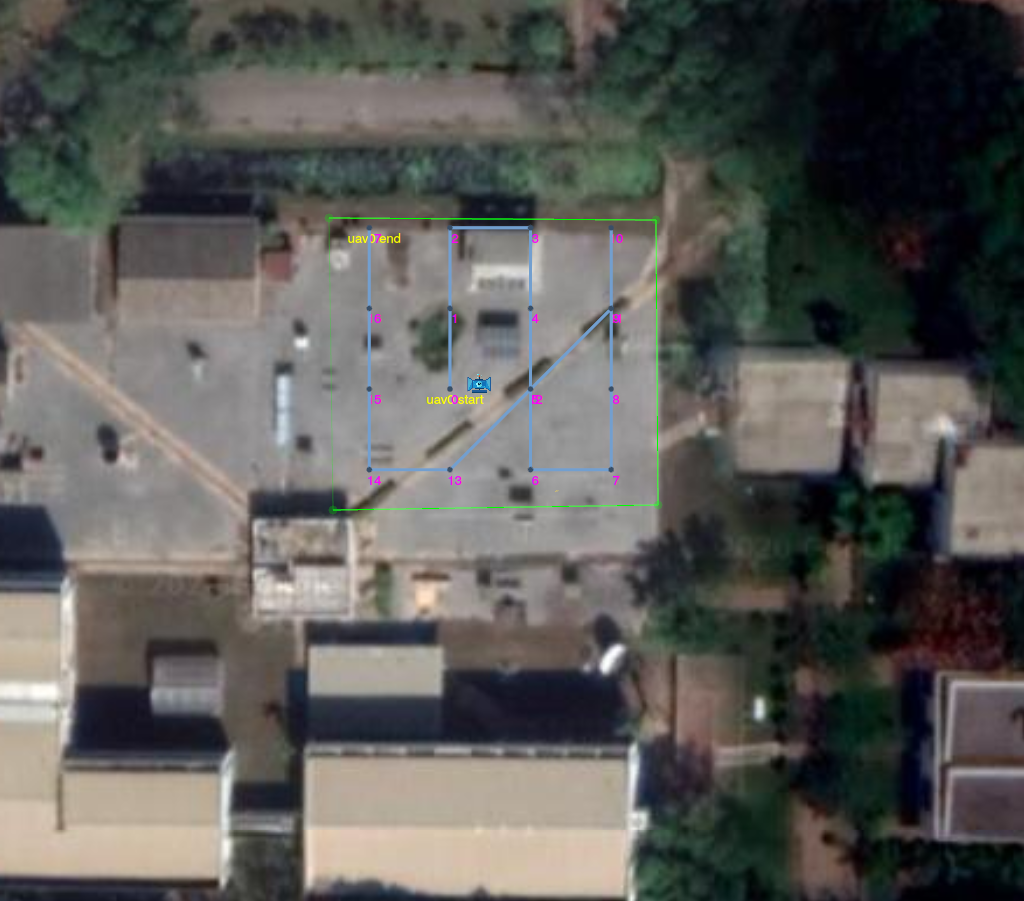
\includegraphics[width=5in]{figures/experiment/real_mapviz_plan}
	\label{fig:real-path}
\end{figure}

\subsection{Motion Control}
The pegasus\_controller was able to successfully communicate with the pegasus\_com-mander in the drone and control the motion of the drone in off-board mode throughout the experiment. The movement type was set to strafe to reduce the time taken for the mission as the drone would not need to align itself at yaw 0\degree after reaching every viewpoint. The pegasus\_controller was successfully able to calculate the transform between the local map of the drone and the global map after the calibration routine. To ensure the safety of the drone, the system was started with the drone in HOLD mode at 20 meters altitude. There was a slight drift in the position of the drone when it was being set to off-board mode through the companion computer. The actual path of the drone during the mission as reported by GPS data received through the heart beat reply is shown in Figure~\ref{fig:real-gps}. The figure does not show drone returning to its home position after the end of the mission because heart beat message is stopped after the drone has reached and collected image in the last pose of its path. Figure~\ref{fig:q-real-gps} shows the complete GPS path in QGroundControl in a mobile smartphone connected through ESP32 wifi telemetry module attached to the flight controller. The difference between Figure~\ref{fig:real-gps} and \ref{fig:q-real-gps} is that first figure is being reported through the Pegasus heart beat mechanism with an interval of one seconds, while the latter is being published directly by the flight controller.


\begin{figure}
	\centering
	\caption[GPS position reported through Pegasus system.]{\small GPS position reported through Pegasus system.} 
	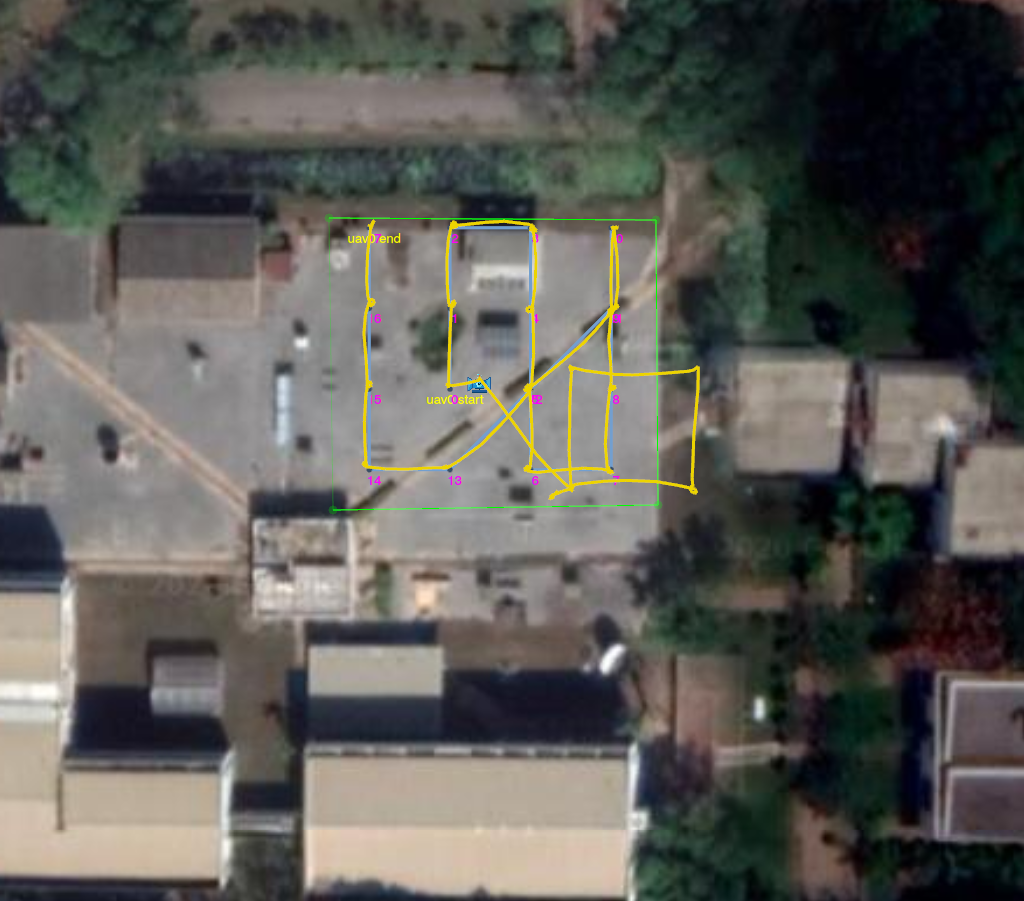
\includegraphics[width=5in]{figures/experiment/real_mapviz_path}
	\label{fig:real-gps}
\end{figure}

\begin{figure}
	\centering
	\caption[GPS position reported through telemetry wifi.]{\small GPS position reported through telemetry WiFi in QGroundControl.} 
	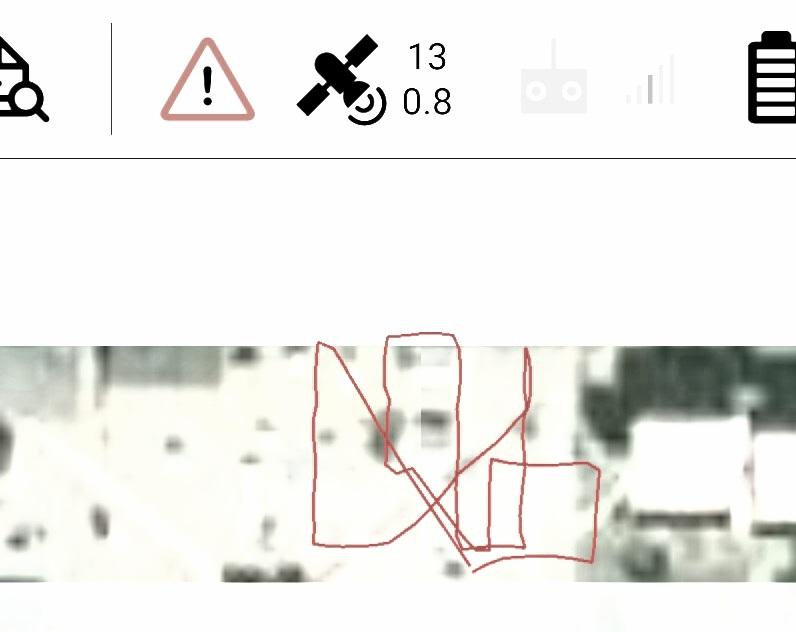
\includegraphics[width=5in]{figures/experiment/q-ground-control}
	\label{fig:q-real-gps}
\end{figure}


\subsection{Result}

The pegasus\_image\_subscriber and pegasus\_image\_publisher successfully acquired 16 images from 16 viewpoints of the mission in real time as shown in Figure~\ref{fig:real-images}. Using an application called photini, the location of the images can be seen in Figure~\ref{fig:exif-real-images}. The GPS EXIF tag from the images show correct viewpoint position.
\begin{figure}
	\centering
	\caption[Images captured by Pegasus in real-time.]{\small Images captured by Pegasus in real-time.} 
	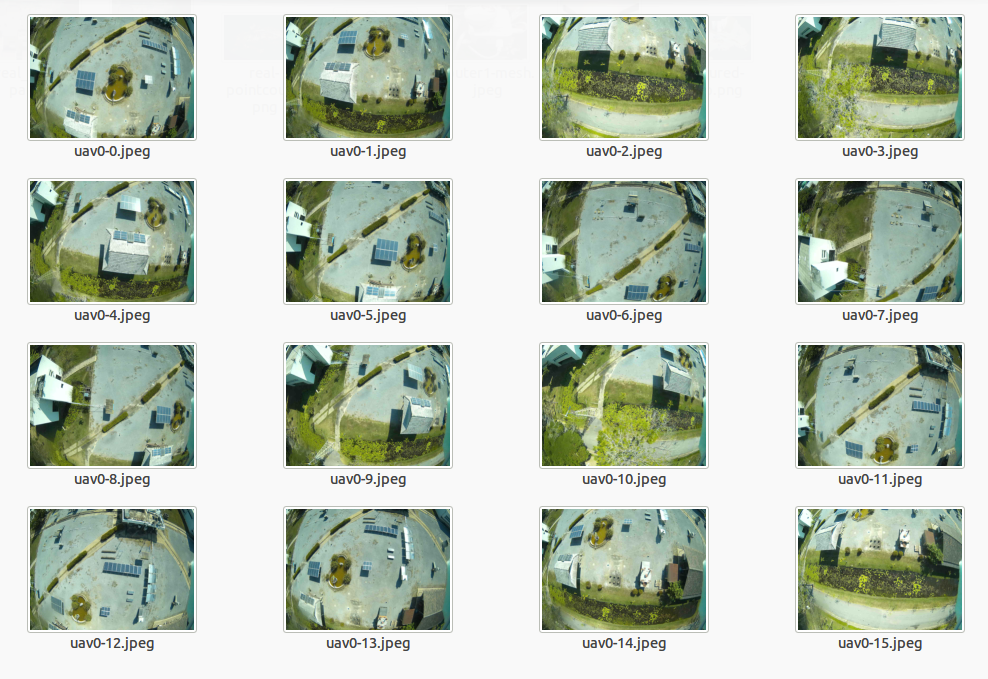
\includegraphics[width=6in]{figures/experiment/real-images}
	\label{fig:real-images}
\end{figure}

\begin{figure}
	\centering
	\caption[Location of images captured in real world experiment.]{\small Location of images captured in real world experiment.} 
	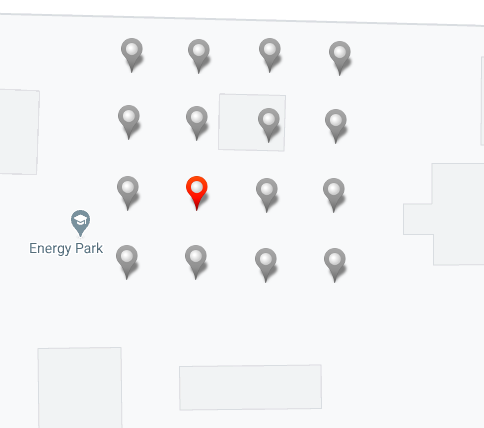
\includegraphics[width=5in]{figures/experiment/real-images-exif-tag}
	\label{fig:exif-real-images}
\end{figure}


The images captured is rectified using pegasus\_image\_rectify using the camera calibration file. Then the rectified images are processed using WebODM.
\begin{itemize}
	\item Figure~\ref{fig:orthophoto-real} shows the generated orthophoto of the region of interest. The orthophoto is skewed from the actual satellite image of the area of interest. It can be seen that the area covered is consistent with the GPS location of the image, but the position of the landmarks are skewed and the image appears smaller than the actual area. Due to the wide field of view of the camera used in the experiment, the image has fish eye distortion. The rectification procedure is not enough to make the images undistorted. It can be seen that in the orthophoto, straight lines are not conserved.
	\item Figure~\ref{fig:real-pointcloud} shows the point cloud for the region of interest. The point cloud is sparse and does not have good definition. 
	\item Figure~\ref{fig:real-textured-map} shows the generated textured mesh of the region of interest. The outside edges are tapering outwards, because of fish eye distortion of the camera used to capture the image and less less overlapping images in the edges of the area of interest.
	\item Figure~\ref{fig:real-camera-position} shows the camera positions determined by ODM over the region of interest. The placement of a few cameras are different from the actual position. The SfM pipeline is not able to properly localize the camera poses due to distortion of the camera in use.
\end{itemize}


\begin{figure}
	\centering
	\caption[Orthophoto of Energy Park.]{\small Orthophoto of Energy Park overlay on top of Google map.} 
	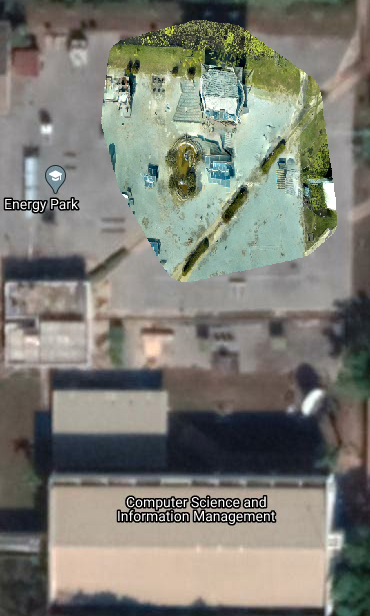
\includegraphics[width=5in]{figures/experiment/orthophoto}
	\label{fig:orthophoto-real}
\end{figure}

\begin{figure}
	\centering
	\caption[Point cloud of Energy Park.]{\small Point cloud of Energy Park.} 
	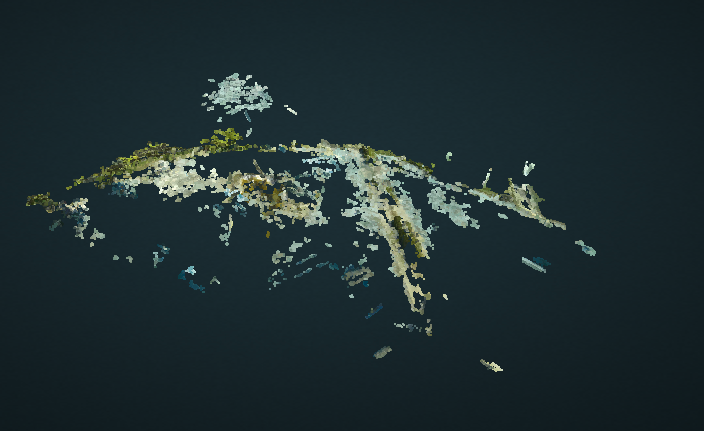
\includegraphics[width=5in]{figures/experiment/point-cloud}
	\label{fig:real-pointcloud}
\end{figure}

\begin{figure}
	\centering
	\caption[Textured mesh of Energy Park.]{\small Textured mesh of Energy Park.} 
	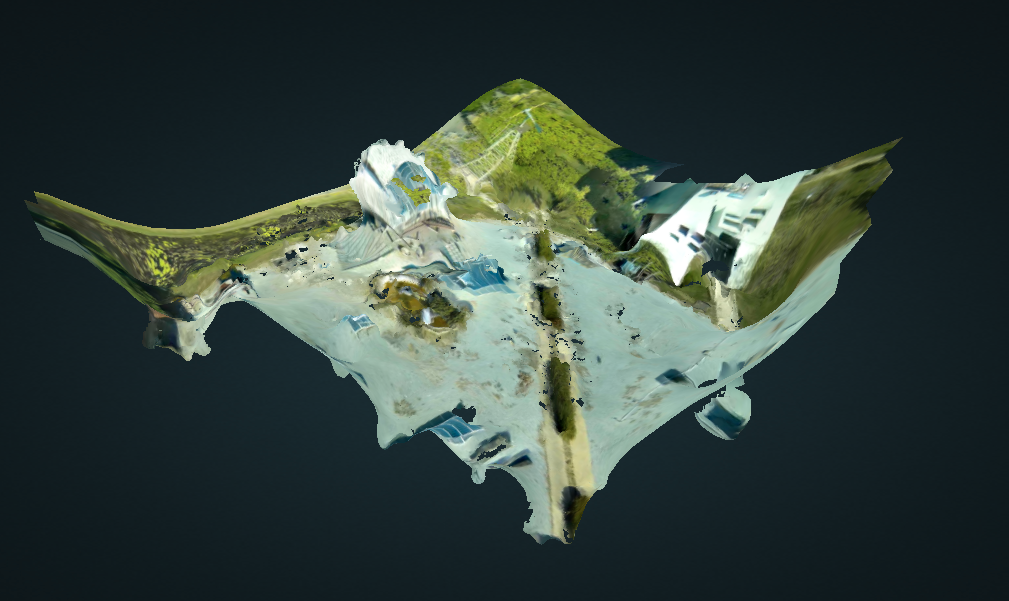
\includegraphics[width=5in]{figures/experiment/textured-mesh-real}
	\label{fig:real-textured-map}
\end{figure}

\begin{figure}
	\centering
	\caption[Camera Position calculated by ODM.]{\small Camera Position calculated by ODM.} 
	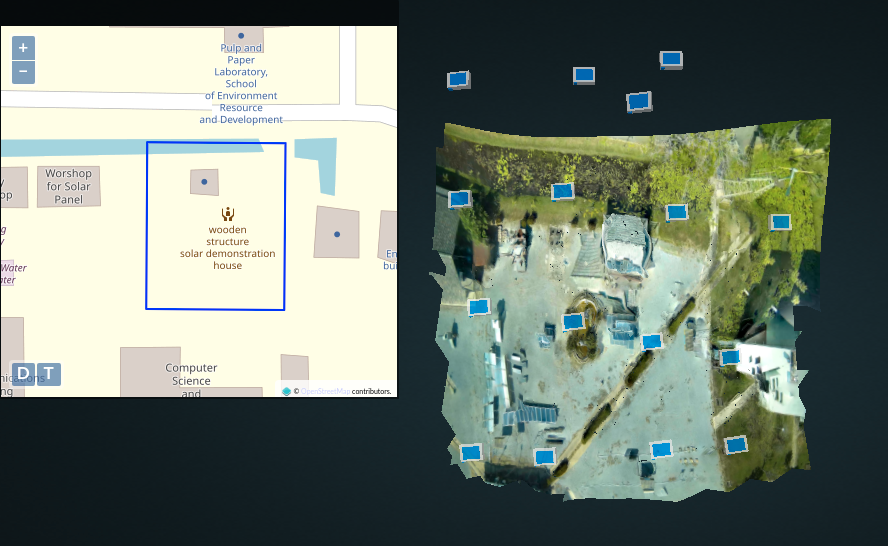
\includegraphics[width=5in]{figures/experiment/camera-position-real}
	\label{fig:real-camera-position}
\end{figure}

\subsection{Summary of Real World Experiment}

The system executes the presentation layer, planning layer, motion control layer and image acquisition layer as expected using wireless mesh network. The map building layer did not provide good quality orthophoto, 3D point cloud and textured mesh. The good quality results of the simulation where the camera provides images without distortion may point to the fish eye camera mounted on the drone being inadequate for our experiment.


\section{Simulation}

Simulation is run on the Gazebo world shown in Figure~\ref{fig:sim-world}. The simulation experiment uses three drones. 

\begin{figure}
	\centering
	\caption[Gazebo simulation world.]{\small Gazebo simulation world 
		(a) Top View. (b) Side View. }
	\subfloat[]{%
		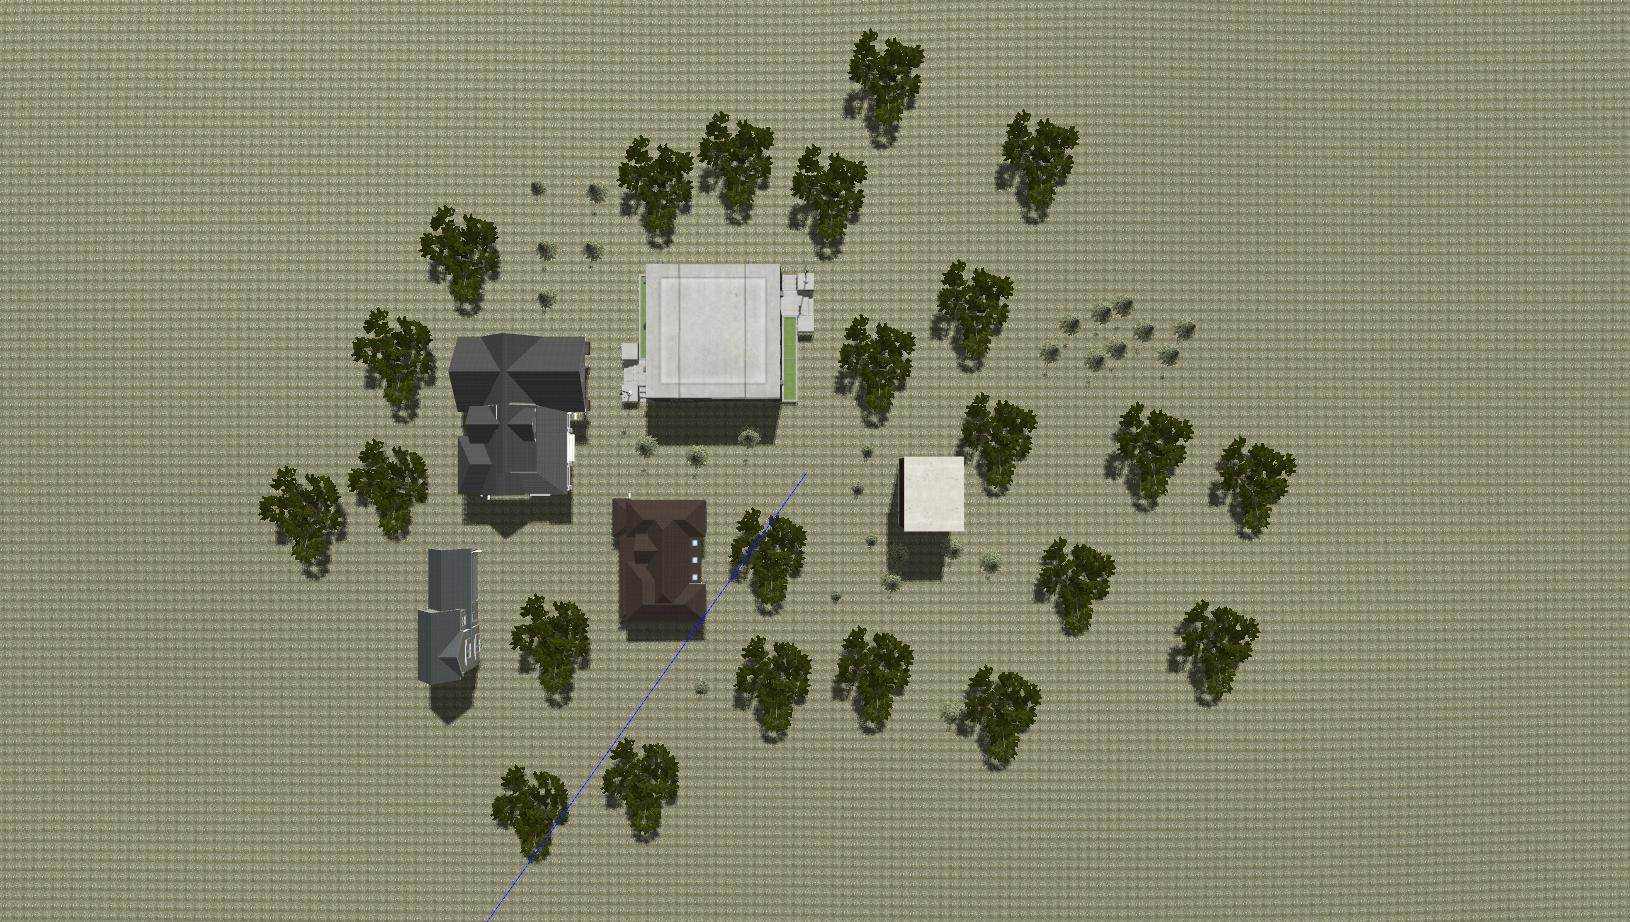
\includegraphics[width=5in]{figures/experiment/sim-world1}
	}
	
	\subfloat[]{%
		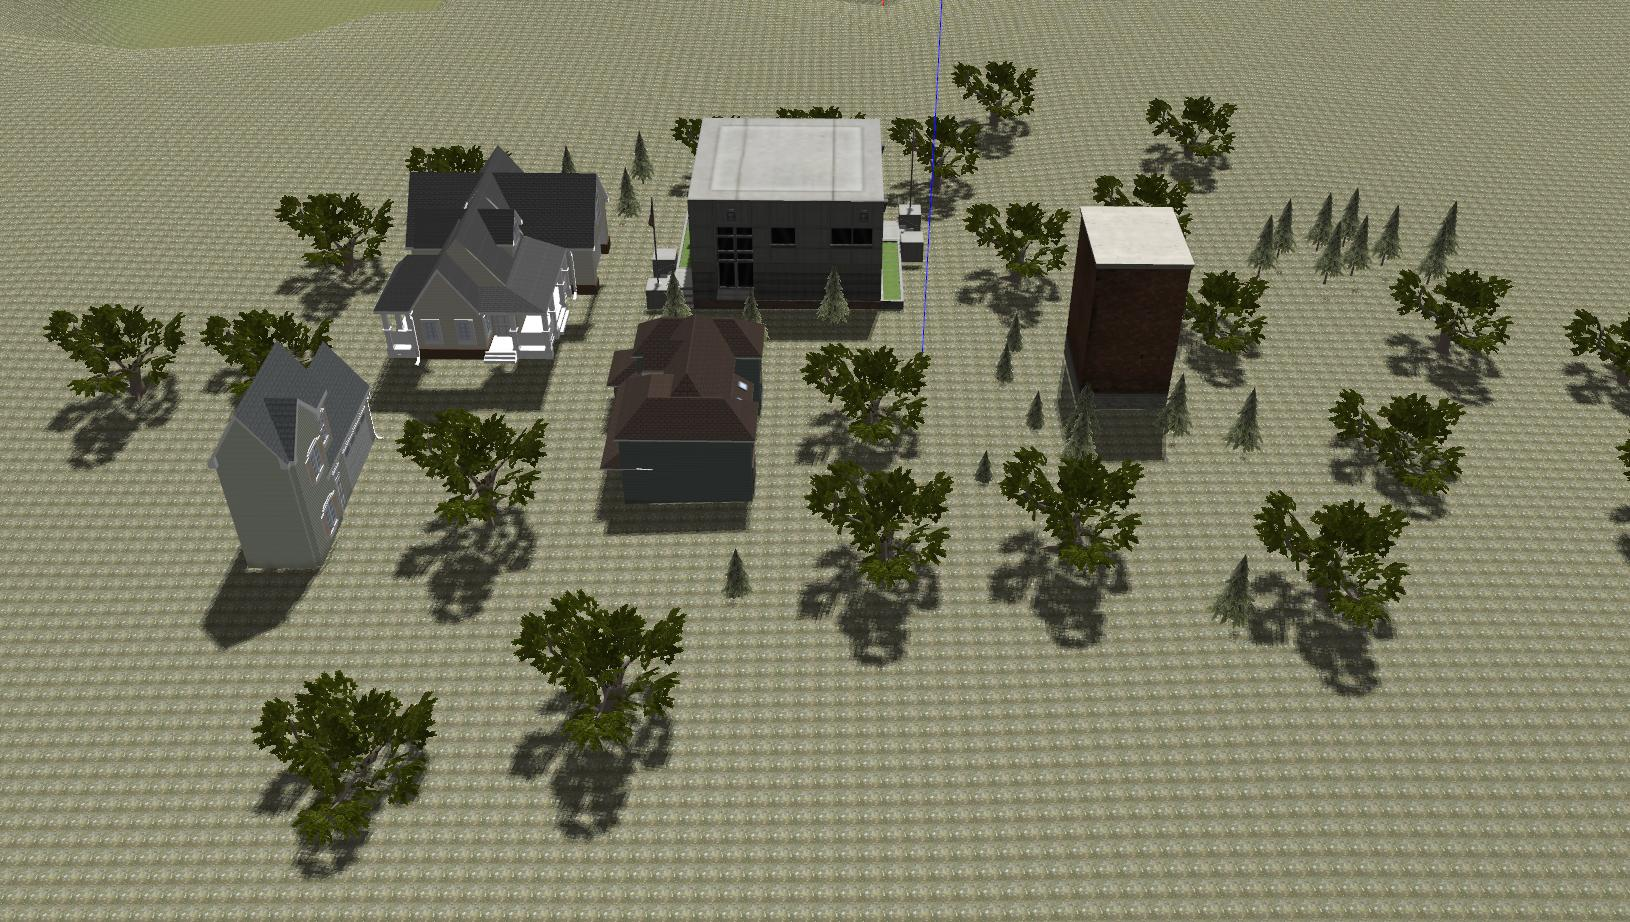
\includegraphics[width=5in]{figures/experiment/sim-world2}%
	}
	\label{fig:sim-world}
\end{figure}

\subsection{Simulated Network Configuration}

All the network packets was routed though ns-3. The OLSR messages' interval for the simulated network is given in Table~\ref{tab:sim-olsr-setting}. Ns-3 was configured to have one GCS node and three drone nodes. Therefore the GCS had a total of six udp sockets to control the system of three drones. The pegasus-net-sim ns-3 simulator was configured as follows:

\begin{verbatim}
std::map<std::string, std::vector<PegasusPortConfig>> 
PegasusConfig::m_config {
  {
    "iris_0", {
      {5444, 4444, 3444},
      {7300, 7400, 7200},
     }
  },
  {
    "iris_1", {
      {5445, 4445, 3445},
      {7301, 7401, 7201},
     }
  },
  {
    "iris_2", {
      {5446, 4446, 3446},
      {7302, 7402, 7202},
     }
  },
  {
    CONTROL_STATION_STR , {
      {3444, 6444, 5444},
      {7200, 8200, 7300},
      {3445, 6445, 5445},
      {7201, 8201, 7301},
      {3446, 6446, 5446},
      {7202, 8202, 7302},
    }
  },
};
\end{verbatim}


\begin{table}[h!]
	\caption[OLSR messsages' interval parameters for simulated experiment.]{OLSR messages' interval parameters for simulated experiment.}
	\begin{center}
		\begin{tabular}{c|c}
			\hline Message & Interval\\ \hline \hline
			Hello & 2 sec \\ \hline
			TC & 5 sec \\ \hline 
			MID & 5 sec  \\ \hline 
			HNA & 5 sec \\ \hline
		\end{tabular}
	\end{center}
	\label{tab:sim-olsr-setting}
\end{table}

\subsection{Automated Planning}
The area of interest was larger than the real world experiment and utilized three drones instead of one, and had more viewpoints. The operational height for the simulation was set at 30 meters. The grid size was set at 10 meters. The mesh range was set to 40 meters. The approximate area to cover was 50 by 55 meters. Planning required 3.74 seconds. Results of planning are given in Table~\ref{tab:simulated-planning}. The path planned by the planner is shown in Figure~\ref{fig:simulated-plan}. The total number of viewpoints is 25. The three drones cumulatively covered 32 viewpoints. Therefore, seven viewpoints were visited more than once. 

\begin{table}[t]
	\caption[Result of \texttt{pegasus\_planner} in simulated experiment with three drones.]{\small Result of \texttt{pegasus\_planner} in simulated experiment with three drones.}
	\begin{center}
		\begin{tabular}{c|c|c|c}
			\hline Type & Number of Drones & Viewpoints Generated & Path Size \\ \hline \hline
			Simulation & 3 & 25 & 11, 11, 10 \\ \hline
		\end{tabular}
	\end{center}
	\label{tab:simulated-planning}
\end{table}

\begin{figure}
	\centering
	\caption[Paths generated for three drones in simulation experiment.]{\small Paths generated for three drones in simulation experiment.} 
	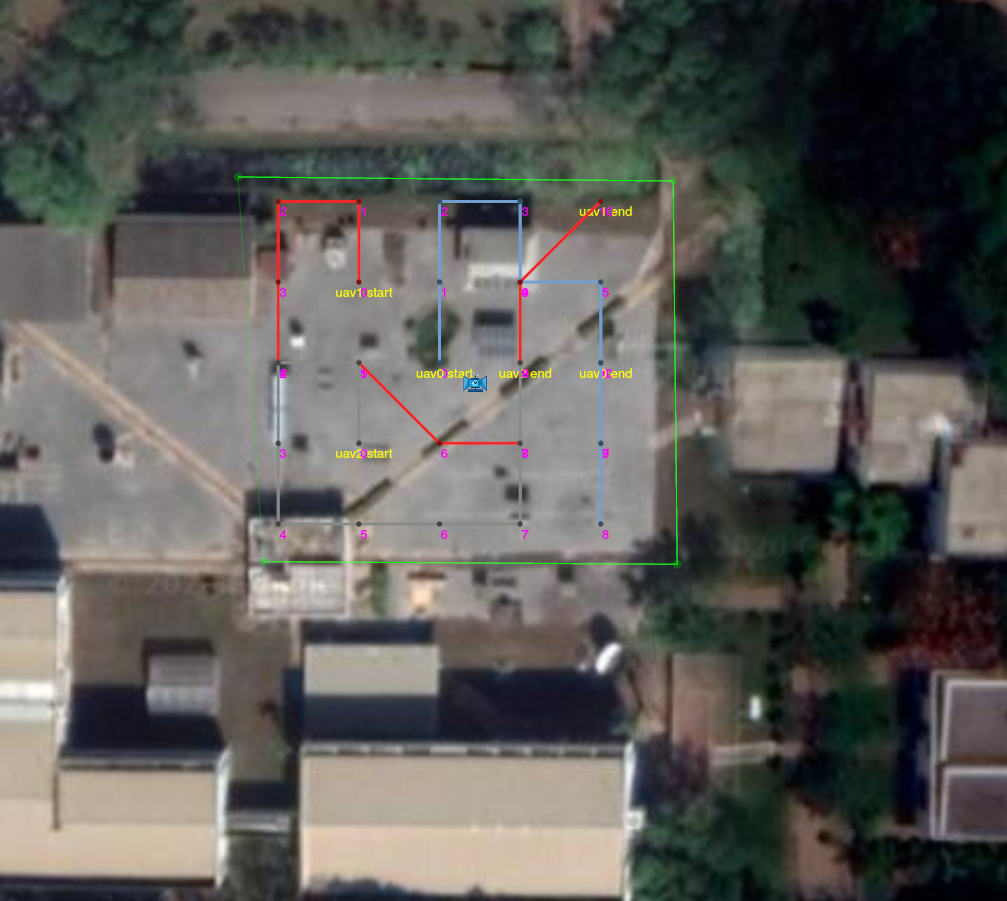
\includegraphics[width=5in]{figures/experiment/simulated-plan}
	\label{fig:simulated-plan}
\end{figure}

\subsection{Motion Control}
The pegasus\_controller was able to control three drones at once though the pegasus\_comman-der process running on each drone. The transformations between the local maps of each drones and the global map were successfully calculated. Pegasus\_controller was able to successfully carry out the coordinated mission without the drones colliding with each other.  The paths taken by the drones are shown in Figure~\ref{fig:simulated-path}. The system never lost mesh connectivity during the mission.

\begin{figure}
	\centering
	\caption[The paths followed by the drones as reported through the simulated GPS.]{\small The paths followed by the drones as reported through the simulated GPS.} 
	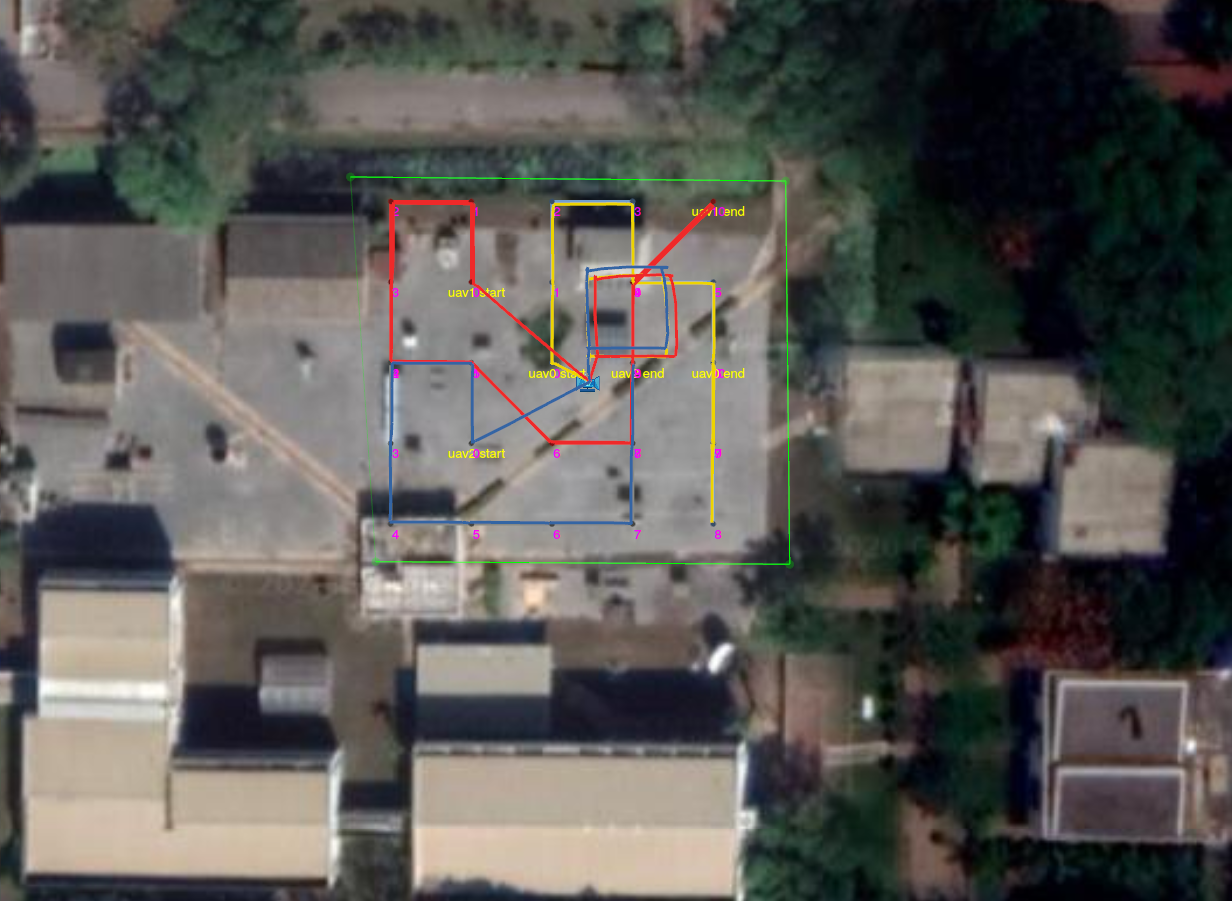
\includegraphics[width=5in]{figures/experiment/simulated-path}
	\label{fig:simulated-path}
\end{figure}

\subsection{Results}
Thirty images were acquired from the three drones in real time. The images were captured with the gst (gstreamer) camera plugin for Gazebo without any distortion. The captured images are shown in Figure~\ref{fig:simulated-images}. The position of the camera for each image as described by the EXIF tag is shown in Figure~\ref{fig:simulated-images-position}. This corresponds with the positions of the viewpoints.
\begin{figure}
	\centering
	\caption[The images captures in real time during simulation.]{\small The images captured in real time during simulation.} 
	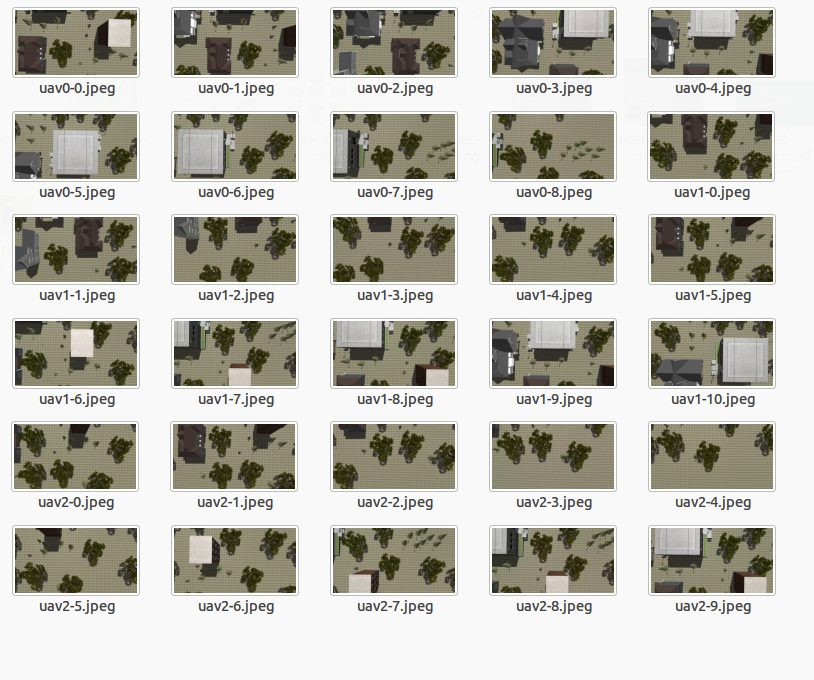
\includegraphics[width=6in]{figures/experiment/simulated-images}
	\label{fig:simulated-images}
\end{figure}

\begin{figure}
	\centering
	\caption[The GPS location of the images captured during simulation.]{\small The GPS location of the images captured during simulation.} 
	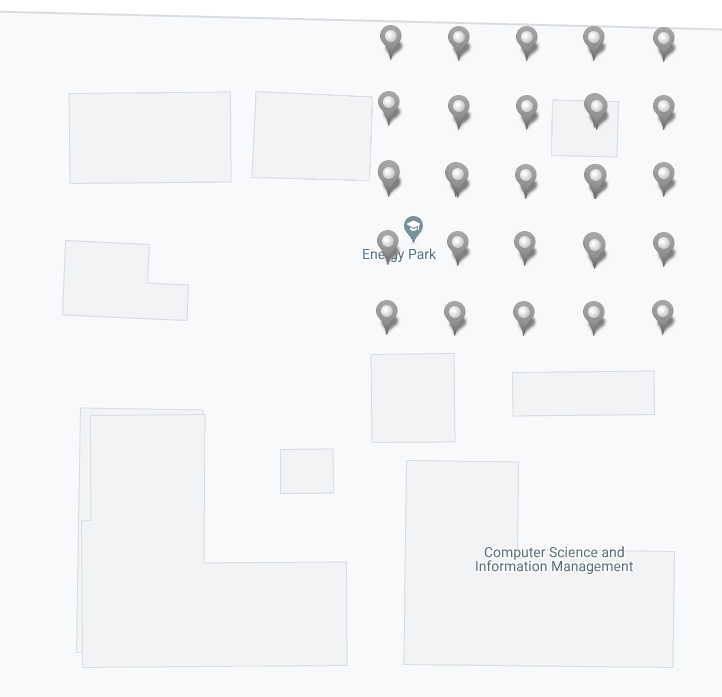
\includegraphics[width=5in]{figures/experiment/simulated-image-position}
	\label{fig:simulated-images-position}
\end{figure}

The network traffic and the ODM outputs are analyzed for the simulation.

\subsubsection{Network Properties}
The traffic in the simulated network was captured in pcap format, then the Wireshark application was used to analyze the traffic. The distribution of packet size is given in Figure~\ref{fig:packet-size-chart}. There were a total of 217,475 packets. 114,551 (52.7\%) of the packets were either IEEE 802.11 frame control or management packets. 59,120 (27.2\%) of the packets were OLSR packets. 43,716  (20.1\%) of the packets were generated by the system. Frame control packets are 14 bytes, and management packets have a size of 65 to 75 bytes. OLSR packets have sizes between 98 and 122 bytes. The Pegasus system generated packets of minimum size 99 to a maximum of 1046 bytes. Figure~\ref{fig:packet-percentage} shows that the Pegasus system was responsible for the least amount of packets; most of of the packets in the network are OLSR and IEEE 802.11 overhead.
The Pegasus system generates two types of packets, motion control and image acquisition packets.  Figures~\ref{fig:pegasus-packet-distribution} and ~\ref{fig:pegasus-packet-distribution-size} show the packet count and megabytes transferred between the GCS and the drones during the simulation. The motion control packets are in the range of kilobytes and did not put any load on the system. The image acquisition layer generated a total of 21.8 megabytes to transfer thirty images. The image acquisition layer data depends upon the resolution of the cameras used, hence higher resolution cameras will generate more packets. The cumulative size of the thirty images stored at the GCS was 18.6 megabytes. The image acquisition layer generated a total of 3.2 megabytes as overhead data.


\begin{figure}
	\centering
	\caption[Packet size and type distribution in simulation network.]{\small Packet size and type distribution in simulated network. (a) The distribution of packet size. (b) The distribution of packet type. }
	\subfloat[]{%
		\label{fig:packet-size-chart}
		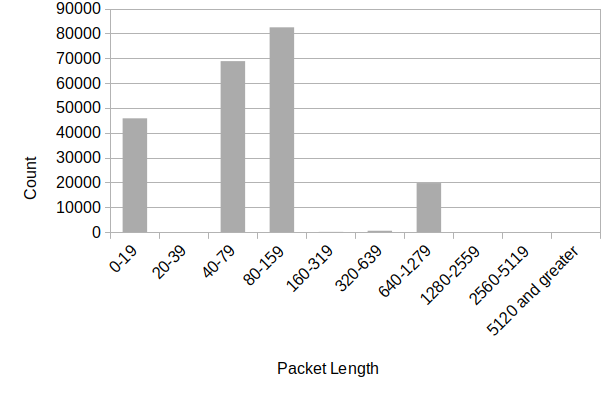
\includegraphics[width=5in]{figures/experiment/packet-size-chart}
	}

	\subfloat[]{%
		\label{fig:packet-percentage}
		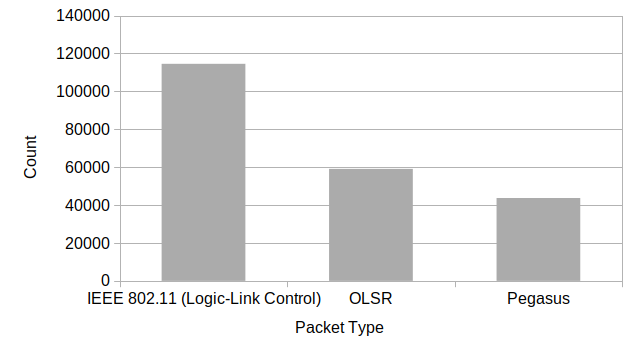
\includegraphics[width=5in]{figures/experiment/percentage-packet}%
	}
	\label{fig:simulated-network-properties-distribution}
\end{figure}

\begin{figure}
	\centering
	\caption[Packets generated by \texttt{Pegasus} system between the GCS and the simulated drones.]{\small Packets generated by \texttt{Pegasus} system between the GCS and the simulated drones. (a) Based on packet count. (b) Based on megabytes transferred. }
	\subfloat[]{%
		\label{fig:pegasus-packet-distribution}
		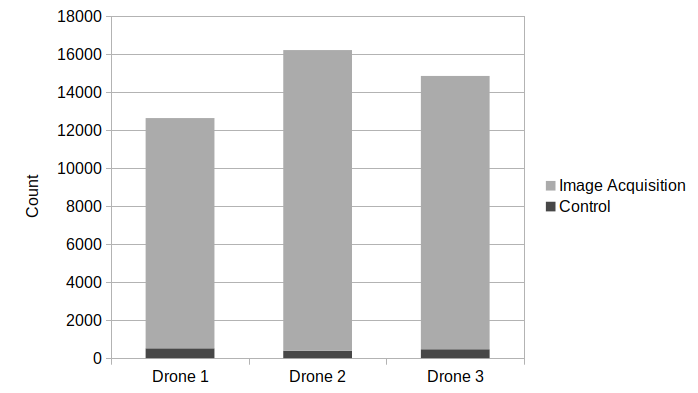
\includegraphics[width=5in]{figures/experiment/pegasus-packet-distribution}
	}

	\subfloat[]{%
		\label{fig:pegasus-packet-distribution-size}
		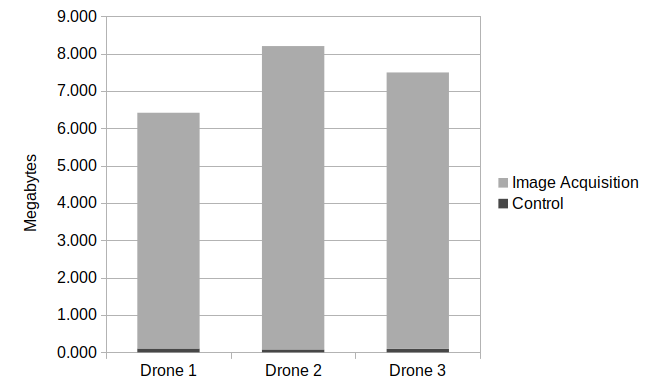
\includegraphics[width=5in]{figures/experiment/pegasus-packet-distribution-size}%
	}
	\label{fig:simulated-network-properties}
\end{figure}


\subsubsection{Map building}
The images did not have distortion, hence they were directly processed using WebODM.
\begin{itemize}
	\item Figure~\ref{fig:orthophoto-simulated} shows the generated orthophoto of the region of interest. The resulting orthophoto is not skewed, and straight lines in the simulated world appear as straight lines in the orthophoto. It covers the entire area of interest selected for the experiment. This result gives us the hint that better cameras with less distortion will result in better orthophotos in real world experiments.
	\item Figure~\ref{fig:simulated-pointcloud} shows the point cloud for the region of interest. The point cloud is sparse but shows better definition than in the real world experiment. This result also provides the insight that less distorted cameras should provide better point clouds.
	\item Figure~\ref{fig:textured-map-simulated} shows the generated textured mesh of the region of interest. The walls of the buildings are not present because the images are taken from a top-view perspective.
	\item Figure~\ref{fig:simulated-camera-position} shows the camera positions determined by ODM over the region of interest, which corresponds to the simulated GPS positions. The SfM pipeline was able to correctly determine the pose of the cameras when the image did not have distortion.  
\end{itemize}

\begin{figure}
	\centering
	\caption[Orthophoto of simulated region of interest.]{\small Orthophoto of simulated region of interest.} 
	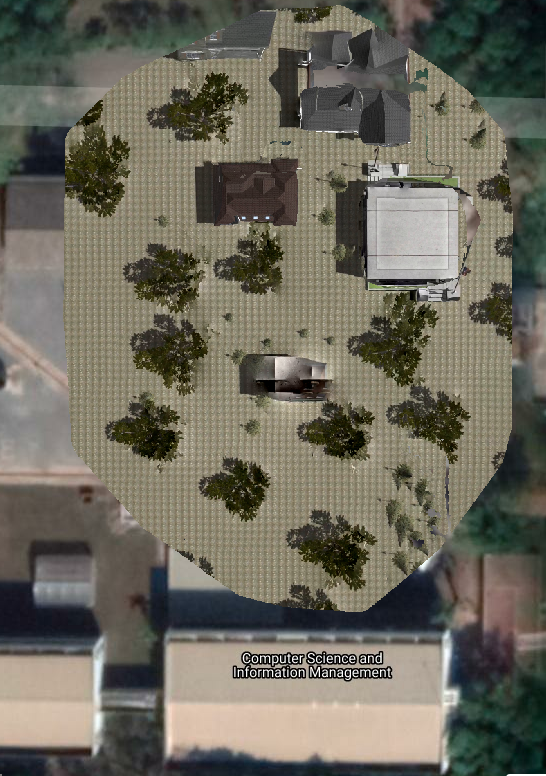
\includegraphics[width=5in]{figures/experiment/orthophoto-simulation}
	\label{fig:orthophoto-simulated}
\end{figure}

\begin{figure}
	\centering
	\caption[Point cloud of simulated region of interest.]{\small Point cloud of simulated region of interest.} 
	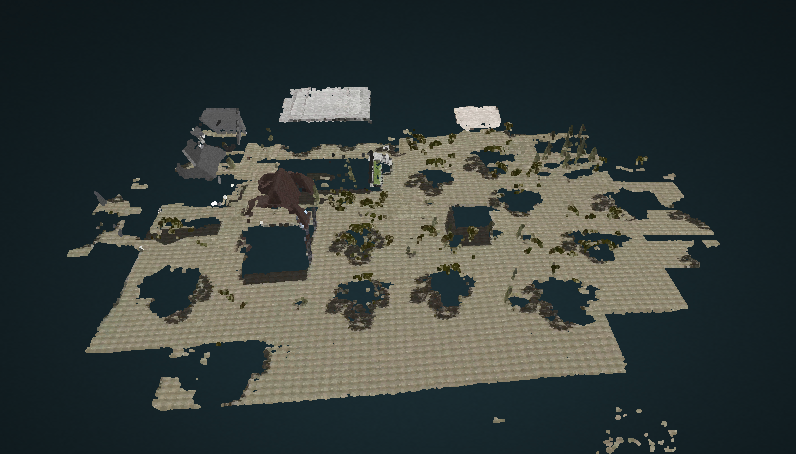
\includegraphics[width=5in]{figures/experiment/simulated-pointcould}
	\label{fig:simulated-pointcloud}
\end{figure}

\begin{figure}
	\centering
	\caption[Textured mesh of simulated region of interest.]{\small Textured mesh of simulated region of interest.} 
	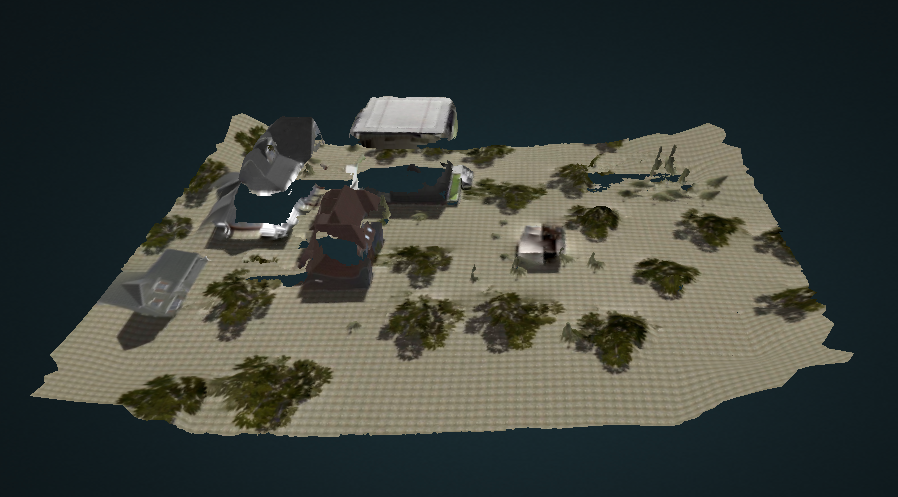
\includegraphics[width=5in]{figures/experiment/textured-simulated}
	\label{fig:textured-map-simulated}
\end{figure}

\begin{figure}
	\centering
	\caption[Position of simulated camera calculated by ODM.]{\small Position of simulated camera calculated by ODM.} 
	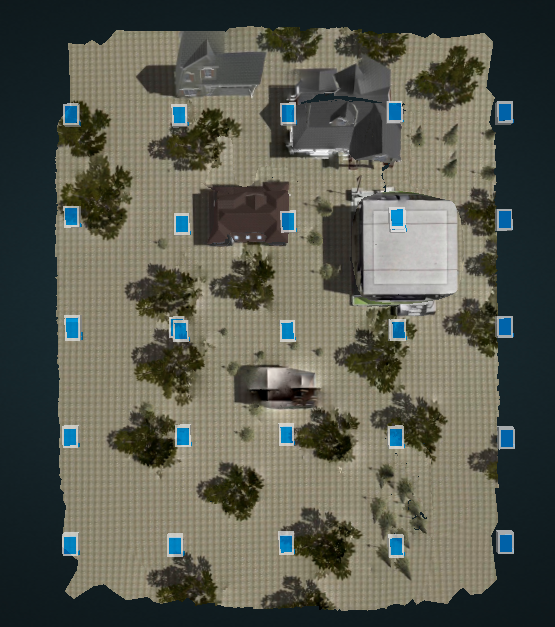
\includegraphics[width=5in]{figures/experiment/simulated-camera}
	\label{fig:simulated-camera-position}
\end{figure}

\subsection{Summary of Simulation Experiment}

The system executed the presentation layer, planning layer, motion control layer, image acquisition layer, and map building layer using three drones. Analysis of the simulated network showed that the IEEE 802.11 logic link layer and OLSR added a great deal of overhead to the system. The networking overhead was actually larger than the actual data generated by the system. The motion control layer generated a small amount of traffic. The simulated cameras provided images without any distortion. The quality of the orthophoto, 3D point cloud and the textured mesh was good in the simulation experiment.

\section{Chapter Summary}
In this chapter, the path planned, the real path taken by the drone, the images acquired by the GCS in real time, and the output of ODM (orthophoto, point cloud and textured mesh) for both the real world and simulation experiments are presented. The distribution of packet size and traffic in the simulated mesh network for the simulation experiment is also described. Overall, the system performs well.


\FloatBarrier